\capitolo{Meccanica delle Vibrazioni}
Ripasso di Meccanica delle Vibrazioni con focus su: oscillatore semplice smorzato, analisi modale di sistemi a più gradi di libertà.

\sezione{Oscillatore Semplice Smorzato}
L'oscillatore semplice smorzato è un modello di corpo, avente una certa massa \(m\) , vincolato tramite un elemento elastico \(k\) e un elemento viscoso \(c\) a telaio.

Per un sistema così fatto è possibile scrivere le 3 equazioni della dinamica:
\begin{itemize}
    \item Equazione di Equilibrio: \(F(t) + F_e(t) + F_v(t) = m \acc{x}(t) \)
    \item Equazione di Legame: \(F_e(t) = -k x(t)\) e \( F_v(t) = -c\dot{x}(t) \)
    \item Equazione di Moto: \(m\acc{x}(t) + c\dot{x}(t) + k x(t) = F(t)\)
\end{itemize}

La soluzione generale dell'equazione differenziale definita dalle equazioni del sistema è dato da soluzione omogenea e soluzione particolare: \(x(t) = x_1(t) + x_2(t)\).

\sottosezione{Soluzione omogenea (Risposta Libera)}
La soluzione di \(m\acc{x}(t)+c\dot{x}(t)+kx(t)=0\), cui si associa il polinomio caratteristico \( \lambda^2 m +\lambda c +k = 0 \) è la soluzione omogenea dell'equazione differenziale. 
Dividendo per la massa si ottengono rispettivamente il fattore di smorzamento e la pulsazione naturale del sistema: \( \epsilon = \frac{c}{2\sqrt{km}} \) e \(\omega_n = \sqrt{\frac{k}{m}}\).
Le radici del polinomio omogeneo associato sono \(\lambda_{1,2} = \epsilon \omega_n \pm \omega_n \sqrt{\epsilon^2 - 1}\), che per i vari \(k>0,m>0,c>0\) permettono di distinguere vari casi:
\begin{enumerate}
    \item \(\epsilon > 1\): Sistema sovrasmorzato, permette di ritornare alla condizione di equilibrio, \(x_1(t) = A_1 e^{\lambda_1t} + A_2 e^{\lambda_2t}\)
    \item \( \epsilon = 1 \): Sistema criticamente smorzato, permette di   ritornare alla condizione di equilibrio il più velocemente possibile senza oscillazioni, \(x_1(t) = (A_1+t A_2) e^{-\omega_n t} \)
    \item \( 0 < \epsilon < 1 \): Sistema sottosmorzato, ritorna alla condizione di equilibrio, ma con oscillazioni, \(x_1(t) = C e^{-\epsilon \omega_n t} \sin{\left(\omega_d t + \Phi \right)}\)
    \item \(\epsilon = 0\): Sistema non smorzato, non c'è ritorno alla condizione di equilibrio, \( x_1(t) = B_1 \cos{\left( \omega_n t \right)} + B_2 \sin{\left( \omega_n t \right)} \)
\end{enumerate}

La soluzione omogenea ha significato di risposta libera del sistema, ossia in condizione di forzante nulla.

\sottosezione{Soluzione particolare (Risposta Forzata)}
La soluzione di \(m\acc{x}(t) + c\dot{x}(t) + k x(t) = F(t)\), per una certa forzante \(F(t)\) è la soluzione particolare  dell'equazione differenziale.
In base al tipo di forzante cambia la soluzione particolare.
Possibili forzanti sono:
\begin{enumerate}
    \item \(F(t) = F_0\) Costante
    \item \(F(t) = F_0 \cos{(\omega t)}\) Armonica
    \item \(F(t+T) = F(t) \) Periodica
    \item \(F(t)\) Generica
\end{enumerate}

\sottosottosezione{Forzante Costante}
La forzante costante rappresenta la risposta al gradino di forza di ampiezza \(F_0\), la soluzione particolare di questa forzante è \(x_2(t) = \frac{F_0}{k}\), ed indica la posizione raggiunta a regime.

\sottosottosezione{Forzante Armonica}
La soluzione particolare, per forzante armonica \(F(t) = F_0 \cos{(\omega t)}\), ha risposta che dipende dalla frequenza della forzante.
Per studiare questa soluzione si passa al campo delle frequenze (ipotesi isofrequenziale) e si utilizza la Frequency Responce Function \( \frac{x_0 e^{i\phi}}{F_0} \), il cui modulo è \( \abs{\frac{x_0 e^{i\phi}}{F_0}} = \frac{1}{k\sqrt{\left[1-\left(\frac{\omega}{\omega_n}\right)^2\right]^2+\left(2\epsilon \frac{\omega}{\omega_n}\right)^2}} \).

Per la FRF si possono andare a verificare condizioni limite:
\begin{itemize}
    \item Quasi Statica: \(\phi\simeq 0\), \(\frac{\omega}{\omega_n} << 0\), in questo caso l'effetto dello smorzatore è irrilevante
    \item Zona di Risonanza\footnote{Tecnicamente la risonanza si ha per \(\omega_r=\omega_n\sqrt{(1-2\epsilon^2)}\), che solitamente è vicino alla pulsazione naturale, ma non sono la stessa cosa.}: \(\phi\simeq -\frac{\pi}{2}\), \(\frac{\omega}{\omega_n} = 1\), in questa condizione forza e velocità hanno la stessa direzione, l'energia in ingresso nel sistema può essere tale da portare a rottura il sistema
    \item Zona Sismografica: \(\phi\simeq -\pi\), \(\frac{\omega}{\omega_n} >> 1\), in questo caso la massa è come se fosse sospesa, \( x_0 = \frac{F_0}{m \omega^2} \)
\end{itemize}

% inserire grafico frf fatto con matlab, credo ci sia uno script del professore

\sottosottosezione{Forzante Periodica}
Una forzante periodica può essere scomposta, tramite serie di Fourier, in una serie di componenti armoniche di periodo multiplo del periodo della fondamentale. La soluzione particolare in questo caso è \(x_2(t) = \frac{A_0}{k} + \sum \abs{\frac{x_0 e^{i\phi}}{F_0}}_{\omega=m\overline{\omega}} A_m \cos{\left( m\overline{\omega} t + \alpha_m + \angle{\frac{x_0 e^{i\phi}}{F_0}}_{\omega=m\overline{\omega}} \right)}\)

\sottosottosezione{Forzante Generica, Risposta Impulsiva}
Teorema: \textit{La trasformata della risposta impulsiva corrisponde alla risposta in frequenza di un oscillatore semplice all'ingresso armonico.}
Questo significa che la risposta in frequenza all'impulso è la FRF: \(H(i\omega) = \frac{X(i\omega)}{F(i\omega)} = \frac{x_0 e^{i\phi}}{F_0}\).
Questo permette di ricavare la FRF a partire da misure con shaker elettrodinamici o martello strumentale.


\sezione{Sbilanciamento Statico}\label{sbilanciamentoStat}
Viene definito sbilanciamento statico \( s=mr \), con \(m\) la massa e \(r\) il raggio tra il centro di massa e il centro geometrico, ed è il decentramento di massa rispetto il centro geometrico. La massa quando soggetta a forzante armonica può portare ad alte vibrazioni e quindi a rottura.
La massa è soggetta ad una forza centrigura \(F_c = m\omega^2 r\), dove \(\omega\) è la velocità angolare, questa forza è composta da due componenti che dipendono dall'istante temporale considerato \(F(t)=F_c \sin{(\omega t)}\).
La componente forzante da tenere presente è quella che si scarica su molla e smorzatore\footnote{L'altra componente si scarica sulle guide.} \( F_\parallel = s\omega^2 \sin{(\omega t)} \).
Passando ai vettori complessi è possibile ricavare il modulo di \(\abs{x_0 e^{i\phi}} = \frac{s}{M}\left(\frac{\omega}{\omega_n}\right)^2 \frac{1}{\sqrt{\left[ 1-\left( \frac{\omega}{\omega_n} \right)^2  \right]^2 + \left( 2\epsilon \frac{\omega}{\omega_n} \right)^2}}\).

\begin{figure}[h]
    \centering
    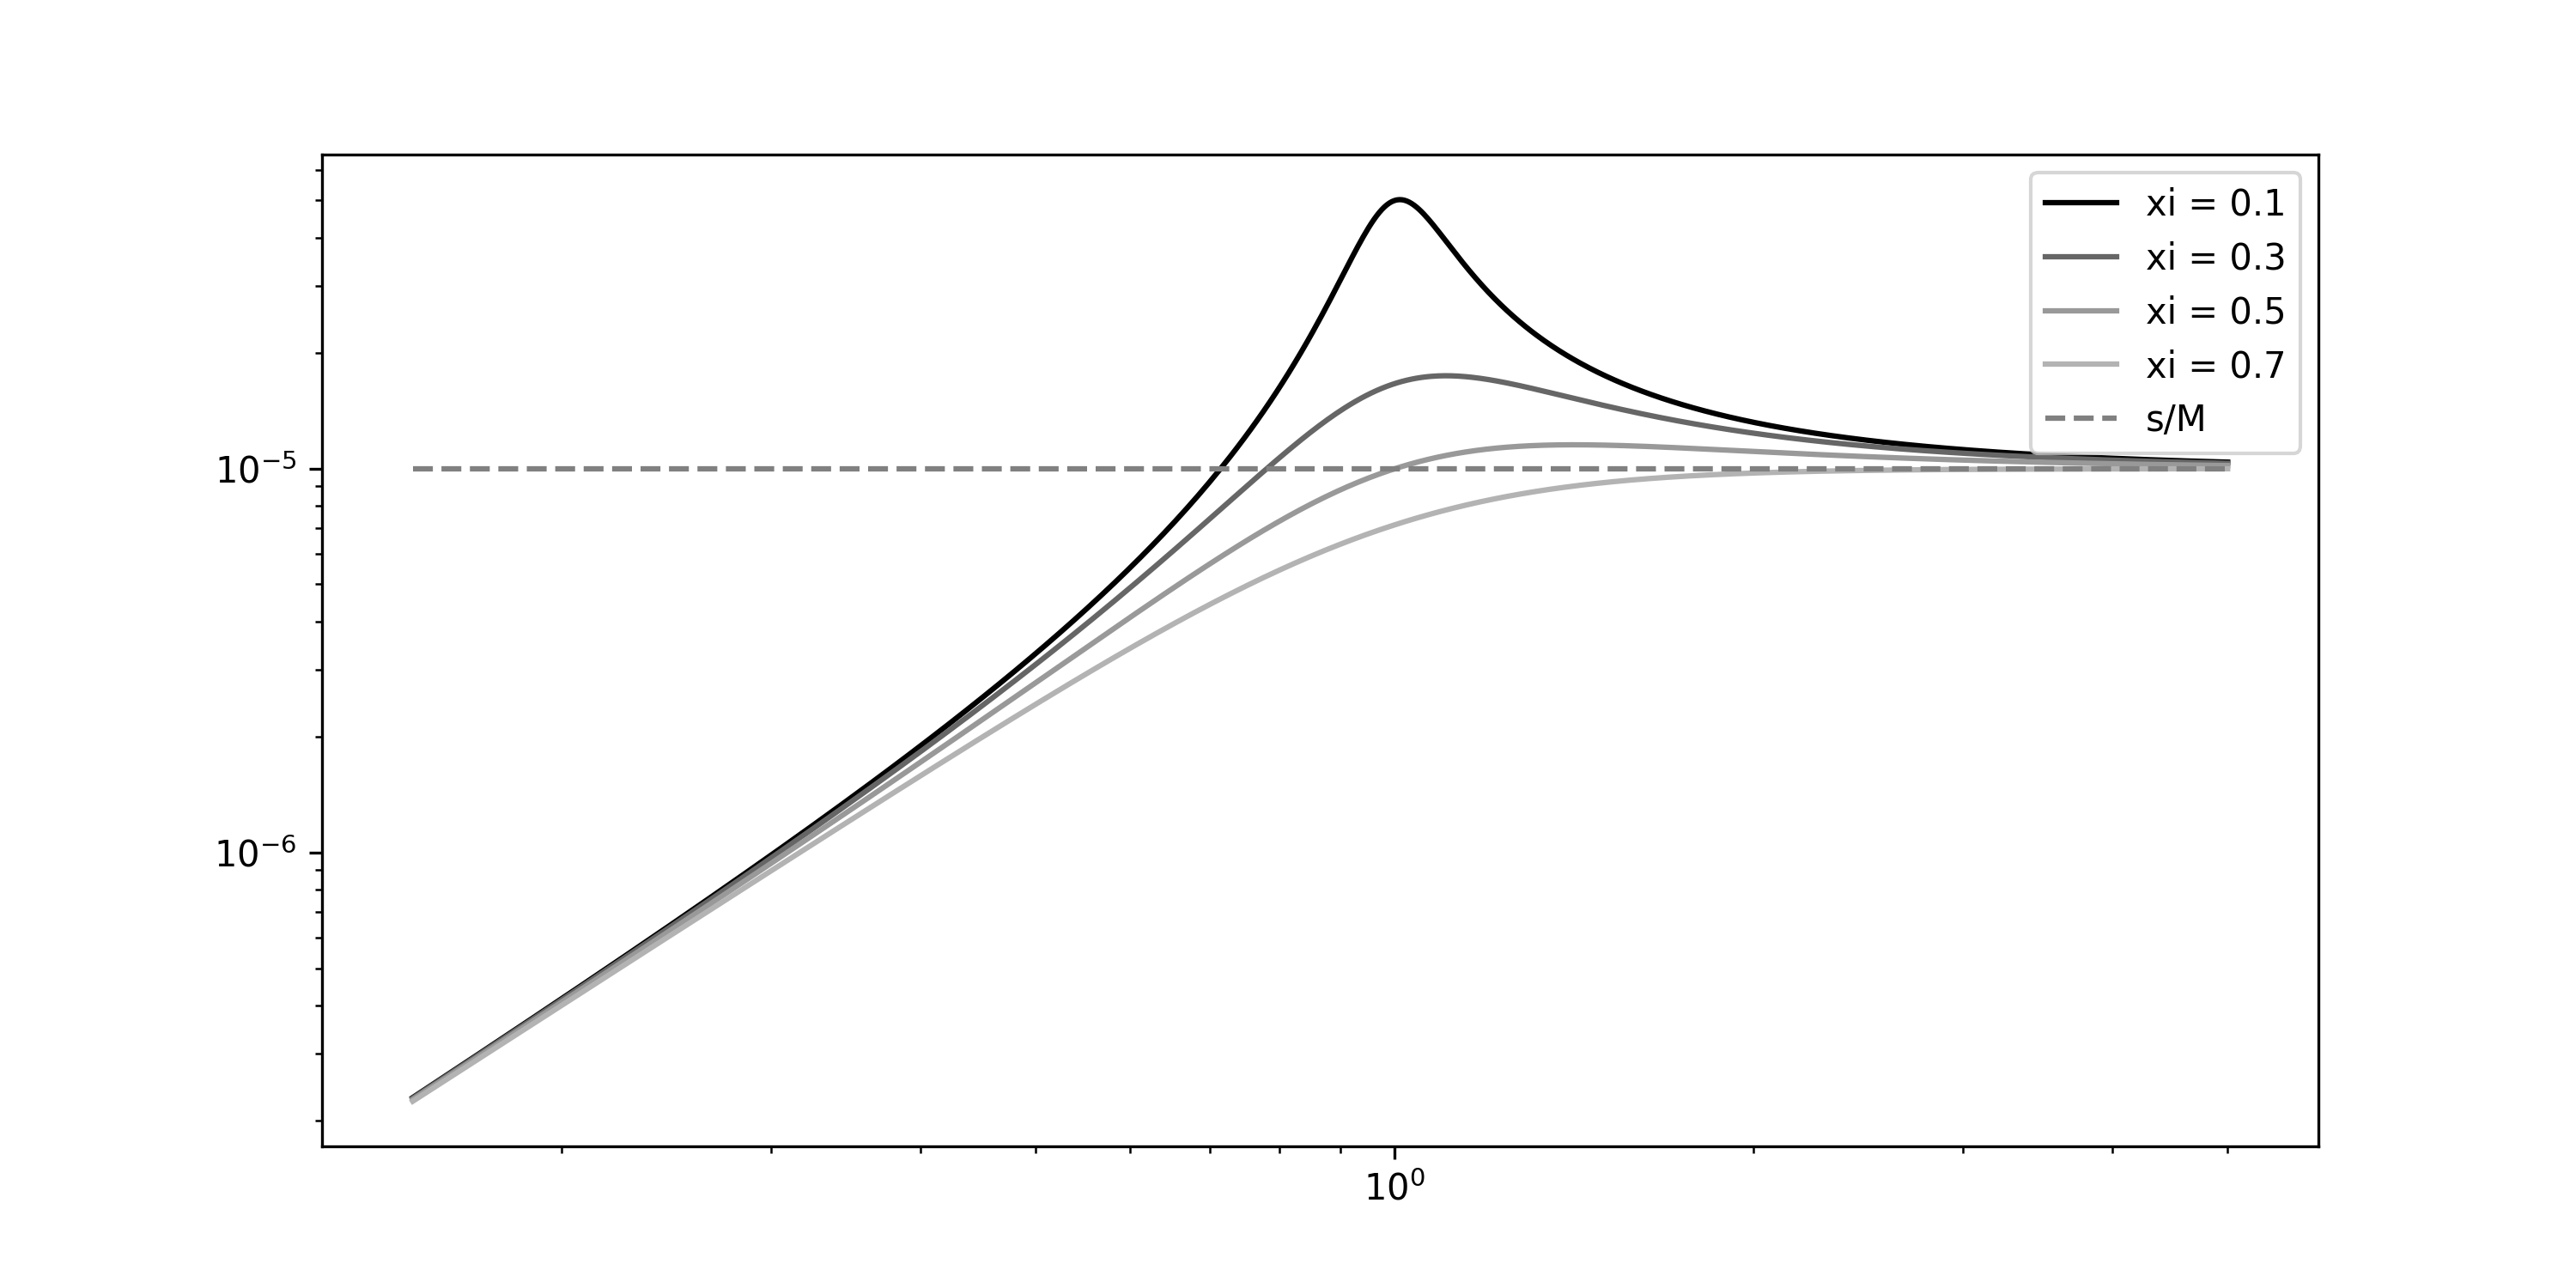
\includegraphics[width=0.5\textwidth]{Immagini/sbilanciamento_statico.png}
    \caption{Sbilanciamento statico \(s=10^{-3}, M=100, \omega_n=1000\)}
\end{figure}

\sezione{Vibrazioni Torsionali}
Si parla di vibrazioni torsionali per un volano collegato ad un estremo di un albero e soggetto ad una coppia \(T(t)\) che provoca una rotazione \(\theta(t)\).
Considerando l'albero privo di massa, assimilabile ad una molla torsionale di rigidezza \(k_T \unitamisura{Nm}{rd} = \frac{I_p^O G}{L}\) dove \(I_p^O = \frac{\pi d^4}{32}\) è il momento di inerzia polare, \(G = \frac{E}{2(1+\nu)}\) modulo elastico tangenziale.
Per la viscosità viene introdotto \(c_T \unitamisura{Nm s}{rd}\).
A questo punto è possibile riportarsi al modello classico di oscillatore semplice smorzato considerando l'inerzia al posto della massa, la rigidezza torsionale e la viscosità torsionale; valgono: \(\omega_n=\sqrt{\frac{K_T}{I^O_p}}\) e \(\epsilon = \frac{c_T}{2\sqrt{K_T I^O_p}}\).

\sezione{Decremento Logaritmico}\label{decr_log}
Il metodo del decremento logaritmico, dedicato a sistemi ad 1gdl oppure aventi \(\xi << 1\), permette, a partire da misure sperimentali, di ricavare pulsazione naturale e smorzamento di un certo sistema.

Considerando una risposta nel tempo del tipo: \(x(t) = e^{-\xi\omega_n t} (B_1 \cos{(\omega_d t)} + B_2 \cos{(\omega_d t)}) \), è possibile fare il rapporto tra due picchi, considerando il periodo di oscillazione pari a \(T_d = \frac{2\pi}{\omega_d}\), che risulta: \(\frac{x_1}{x_2} = \frac{e^{-\xi\omega_n \overline{t}}}{e^{-\xi\omega_n (\overline{t}+T_d)}} = e^{-\xi\omega_n T_d}\).

Il decremento logaritmico è il logaritmo del rapporto appena definito, per cui, noto \(\omega_d = \omega_n\sqrt{1-\xi^2}\), sostituendo, si ottiene:
\[
\delta = \ln{\left(\frac{x_1}{x_2}\right)} =  \xi\frac{2\pi}{\sqrt{1-\xi^2}}
\]

Per valori di \(\xi << 1\), vale \(\xi \simeq \frac{\delta}{2\pi}\).
Utilizzando due picchi non adiacenti, per migliorare la precisione di misura, si ottiene: \(\xi \simeq \frac{\delta}{2 n \pi}\)

\begin{figure}[h]
    \centering
    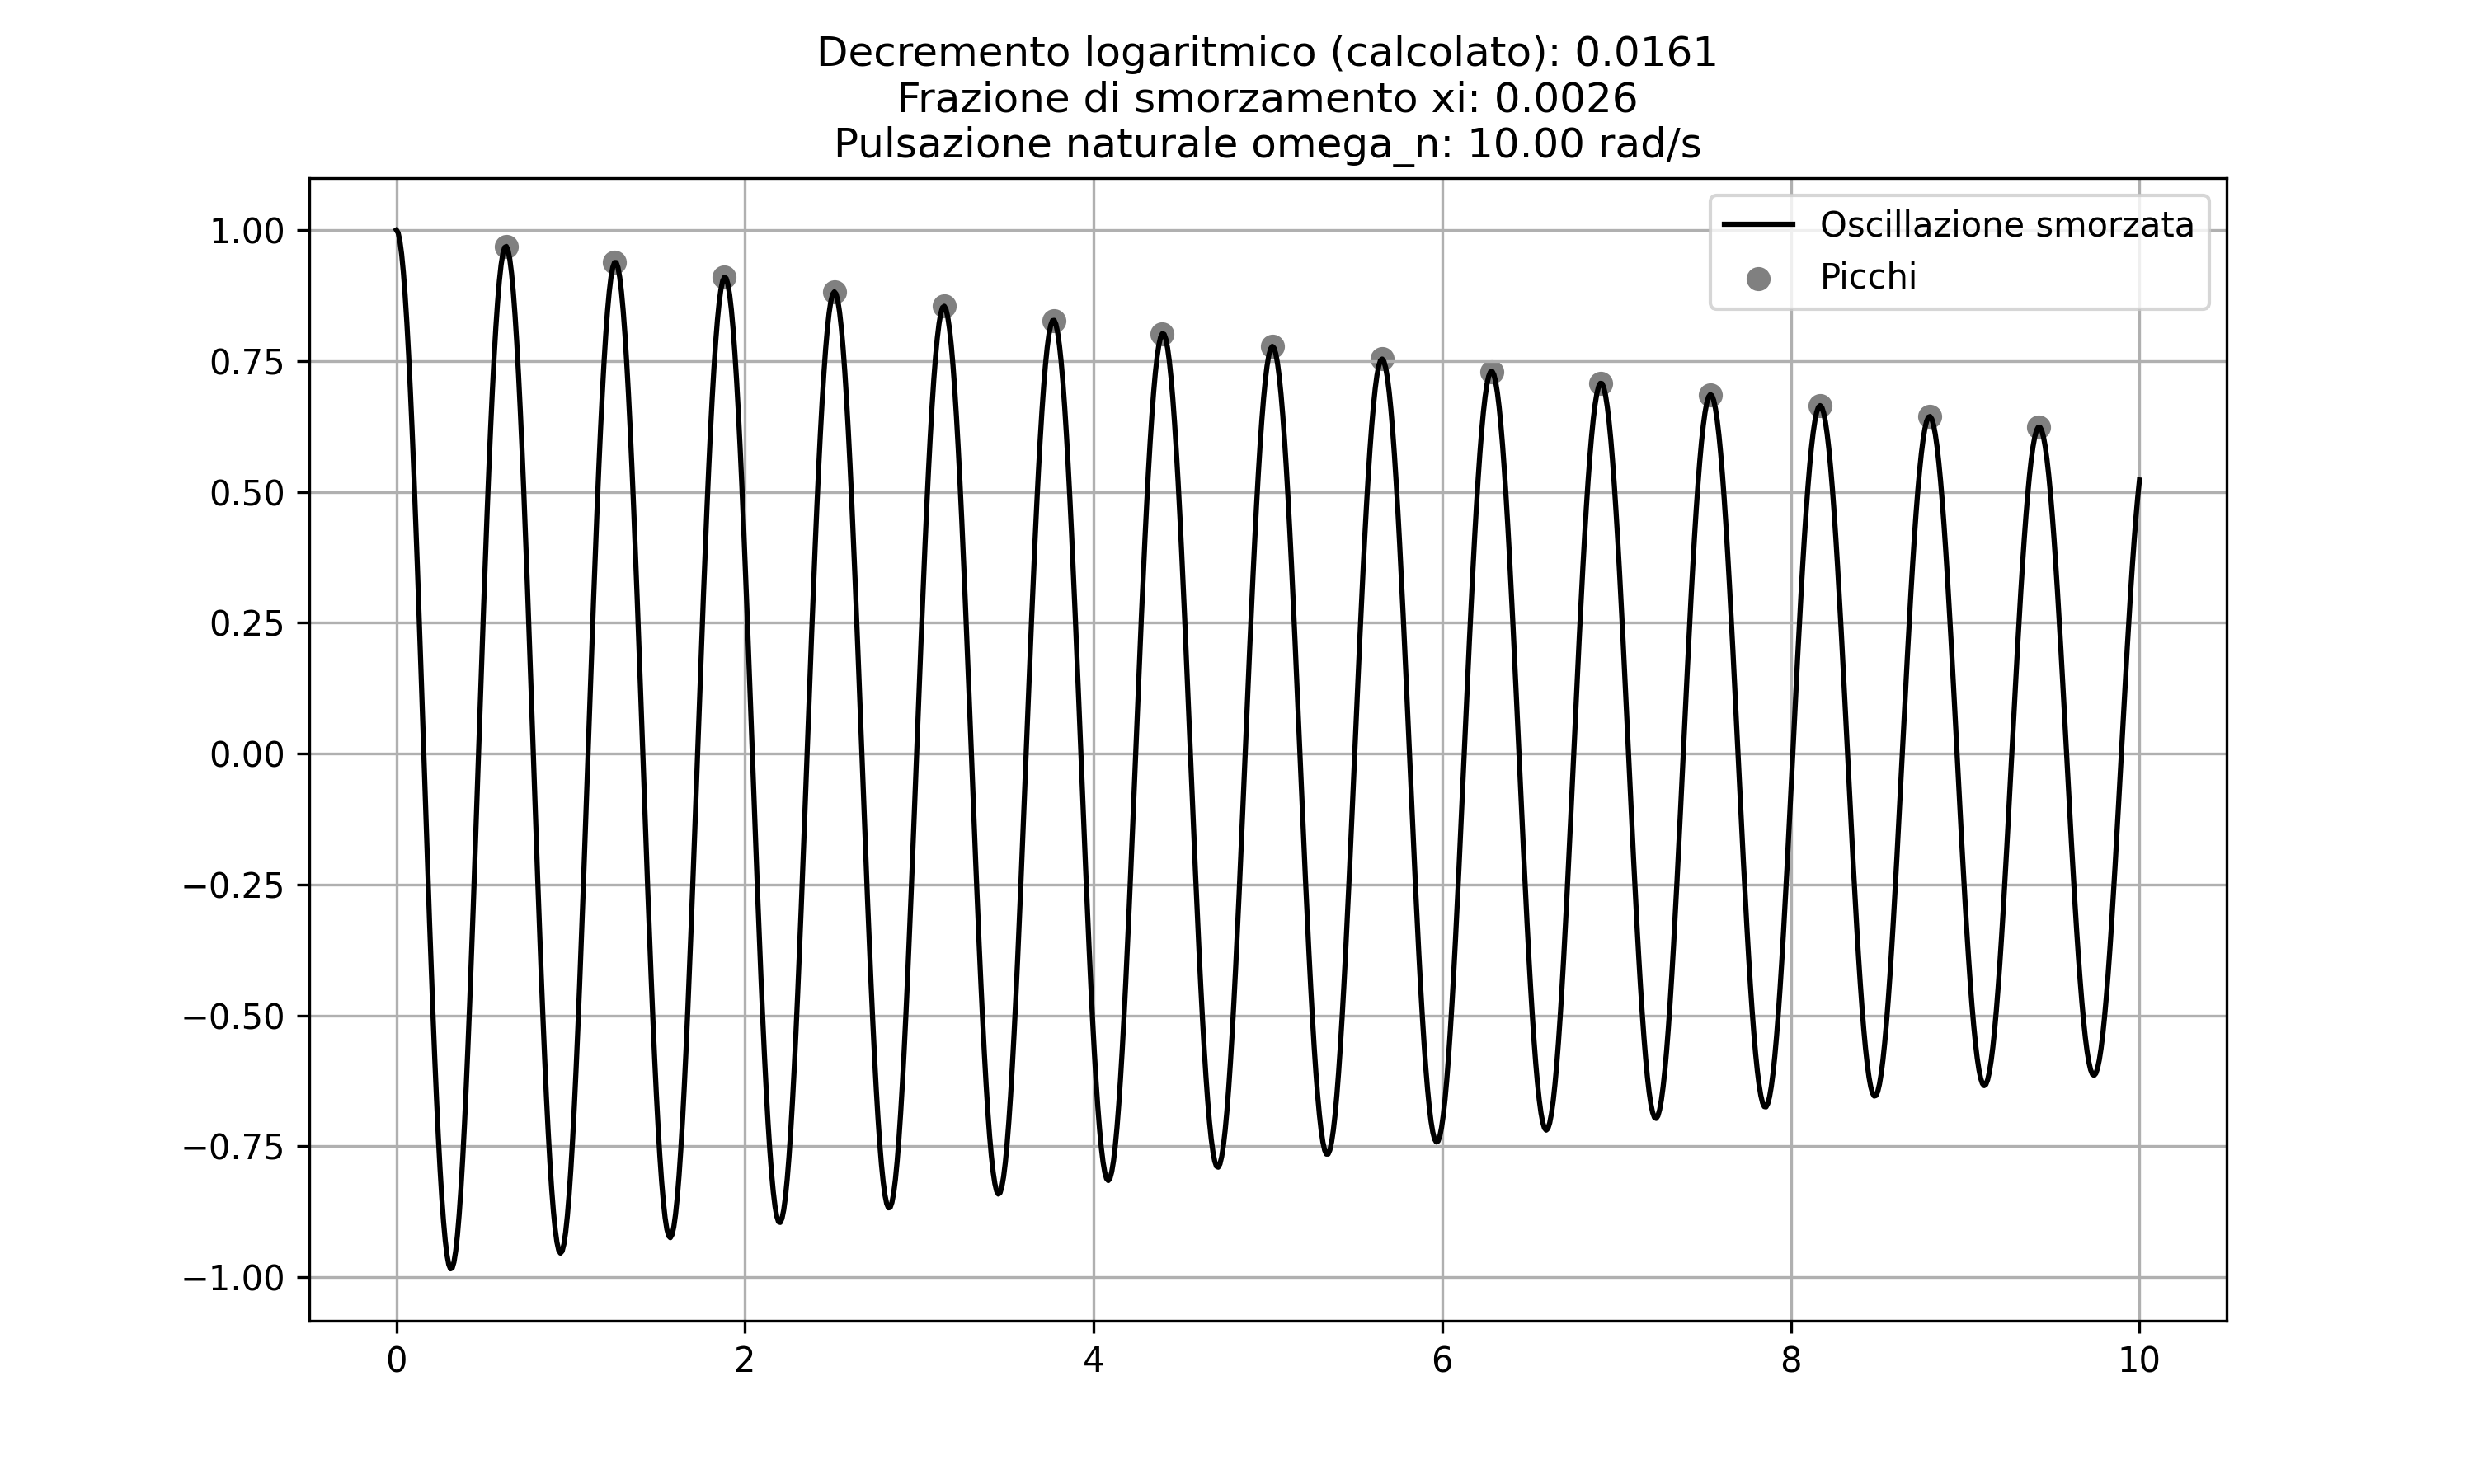
\includegraphics[width=0.5\textwidth]{Immagini/es_decremento_log.png}
    \caption{Esempio calcolo decremento logaritmico}
\end{figure}

\sezione{Analisi Modale}
L'analisi modale consiste nel disaccoppiare le variabili nel sistema di equazioni differenziali.
A partire da un sistema \(\Massa \VettAcc + \left[ c \right] \VettVel + \Rigidezza \VettPos = \left\{ F(t) \right\}\), ignorando l'effetto dello smorzamento, considerando forza esterna nulla, diventa \(\Massa \VettAcc + \Rigidezza \VettPos = 0 \). 
Imponendo una soluzione sincrona del tipo \(\VettPos = \VettU f(t)\), con \(\VettU\) costante nel tempo, e \(f(t)\) che introduce la stessa dipendenza dal tempo per tutti i gdl, significa risolvere \(\Massa \VettU \Ddot{f}(t) + \Rigidezza \VettU f(t) = \VettZero\).
Passando per vettori complessi, manipolando in modo da evidenziare la parte in frequenza\footnote{Avendo imposto una stessa dipendenza da \(f(t)\) per tutti i gdl i vari \(e^{i(\omega t +\phi)}\) si semplificano tra loro.} e quella costante, si ottiene il problema agli autovalori della matrice della dinamica \(\Dinamica\): \(\gamma \VettU = \Dinamica \VettU \), dove \(\Dinamica = \Massa^{-1} \Rigidezza\) e \(\gamma = \omega^2\)
Questo signfica risolvere \(\abs{\Dinamica - \gamma \Identita} = 0\), che non è di soluzione banale.

\sottosezione{Criterio di Normalizzazione}
Per semplificare i calcoli si utilizza un criterio di normalizzazione che permette di ottenere una chiara separazione dei modi (a discapito però del significato fisico).
\begin{itemize}
    \item \(\VettU_i^\top \Massa \VettU_j = \begin{cases} 0 \text{  se } i\neq j \\ 1 \text{  se } i=j \end{cases} \) 
    \item K-ortogonalità \(\VettU_i^\top \Rigidezza \VettU_j = \begin{cases} 0 \text{  se } i\neq j \\ \omega_i^2 \text{  se } i=j \end{cases} \) 
\end{itemize}

\sottosezione{Oscillatore Modale}
Definita la matrice modale \(\Modale\) formata da colonne di  autovettori \(\VettU\), valgono
\begin{itemize}
    \item \(\Modale^\top \Massa \Modale = \Identita \)
    \item \(\Modale^\top \Rigidezza \Modale = \Autoval =  \diag{\omega^2} \)
\end{itemize}

Nota bene, per criterio di normalizzazione che \(\Modale^\top \Massa = \Modale^{-1}\), ossia \(\abs{\Modale} \neq 0\) cioè gli autovalori della matrice della dinamica sono linearmente indipendenti quindi formano una base.
Questo significa che \(\VettPos = \eta_1(t) \VettU_1 + \dots + \eta_n(t) \VettU_n = \Modale \VettModalePos\), che sostituito in \(\Massa \VettAcc + \Rigidezza \VettPos = \left\{ F(t) \right\}\), porta ad un nuovo sistema \(\VettModaleAcc + \Autoval \VettModalePos = \VettModaleForza = \Modale^\top \VettForza \).
Questo nuovo sistema è un oscillatore modale equivalente di massa unitaria che si sposta di \(\eta_i(t)\) e ha una molla equivalente di rigidità \(\omega_i^2\) e forza applicata sulla massa di ampiezza \(l_i(t)\).
Per vedere una forma modale occorre fare una evoluzione libera del sistema con condizioni iniziali pari a uno degli autovalori.

\sottosottosezione{Con Smorzamento}
Nell'oscillatore modale, aggiungere lo smorzamento significa studiare \( \Ddot{\eta}_j(t) + 2\epsilon_j\omega_j \dot{\eta}_j(t) + \omega^2_j \eta_j(t) = l_i(t) \).

\sottosottosezione{Forzante armonica}
Nel caso fossero applicate forzanti armoniche per i vari gdl, aventi stessa pulsazione \(\omega\), ma ampiezze \(F_j\) e fasi \(\phi_j\) differenti , è possibile passare allo studio di oscillatori modali, che possono essere studiati con vettori complessi, e da cui in seguito a opportune manipolazioni  si ottiene: \(\eta_j(i\omega) = \frac{1}{\omega_j^2} \frac{1}{1-\left(\frac{\omega}{\omega_j}\right)^2 + 2\epsilon_j \frac{\omega}{\omega_j}} l_j(i\omega)\).
Dall'oscillatore modale è possibile tornare all'oscillatore semplice: \(\left\{ x(i\omega) \right\} = \Modale \left\{ \eta(i\omega) \right\} = \Modale \left[ T(i\omega) \right] \left\{ L(i\omega) \right\} \), dove \(\left[ T(i\omega) \right]\), infine sostituendo \(\left\{ L(i\omega) \right\} = \Modale^\top \left\{ F(i\omega) \right\}\) e definita la matrice delle risposte in frequenza \( \left[ H(i\omega) \right] = \Modale \left[ T(i\omega) \right] \Modale^\top \), si ottiene \( \left\{ x(i\omega) \right\} = \left[ H(i\omega) \right] \left\{ F(i\omega) \right\} \).
Vale inoltre \(\left[ H(i\omega) \right] = \sum^n_{j=1} \left[ H_j(i\omega) \right] = \sum^n_{j=1} \frac{1}{\omega^2_j} \frac{1}{1-\left(\frac{\omega}{\omega_j}\right)^2 + i2 \epsilon \frac{\omega}{\omega_j}} \VettU_j \VettU_j^\top \).


% inserire parte su analisi modale pag 34-... , 73 o 77 appunti di Enrico

\sottosottosezione{Antirisonanza}\label{antirisonanza}
Con antirisonanza si intendono quelle pulsazioni di un sistema, non smorzato, a più gradi di libertà, tali per cui uno degli elementi della matrice delle risposte in frequenza \(\left[ H(i\omega) \right]\) è nullo.
Il numero di pulsazioni di antirisonanza è pari a \(\text{n gdl} - 1\).

Nel caso di sistema a 2 gdl in figura  \( x_1(i\omega) = h_{11}(i\omega) F_1(i\omega) + h_{12}(i\omega)F_2(i\omega) \), per \( h_{11}(i\omega), F_2(i\omega) = 0\) è come se la massa 1, su cui viene applicata una forzante \(F_1(i\omega)\neq 0\), non si muovesse, quindi fosse, virtualmente, a telaio.

Nel caso di sistemi smorzati non si ha attraversamento per l'asse delle ascisse, quindi non si ha antirisonanza.

\begin{figure}[h]
    \centering
    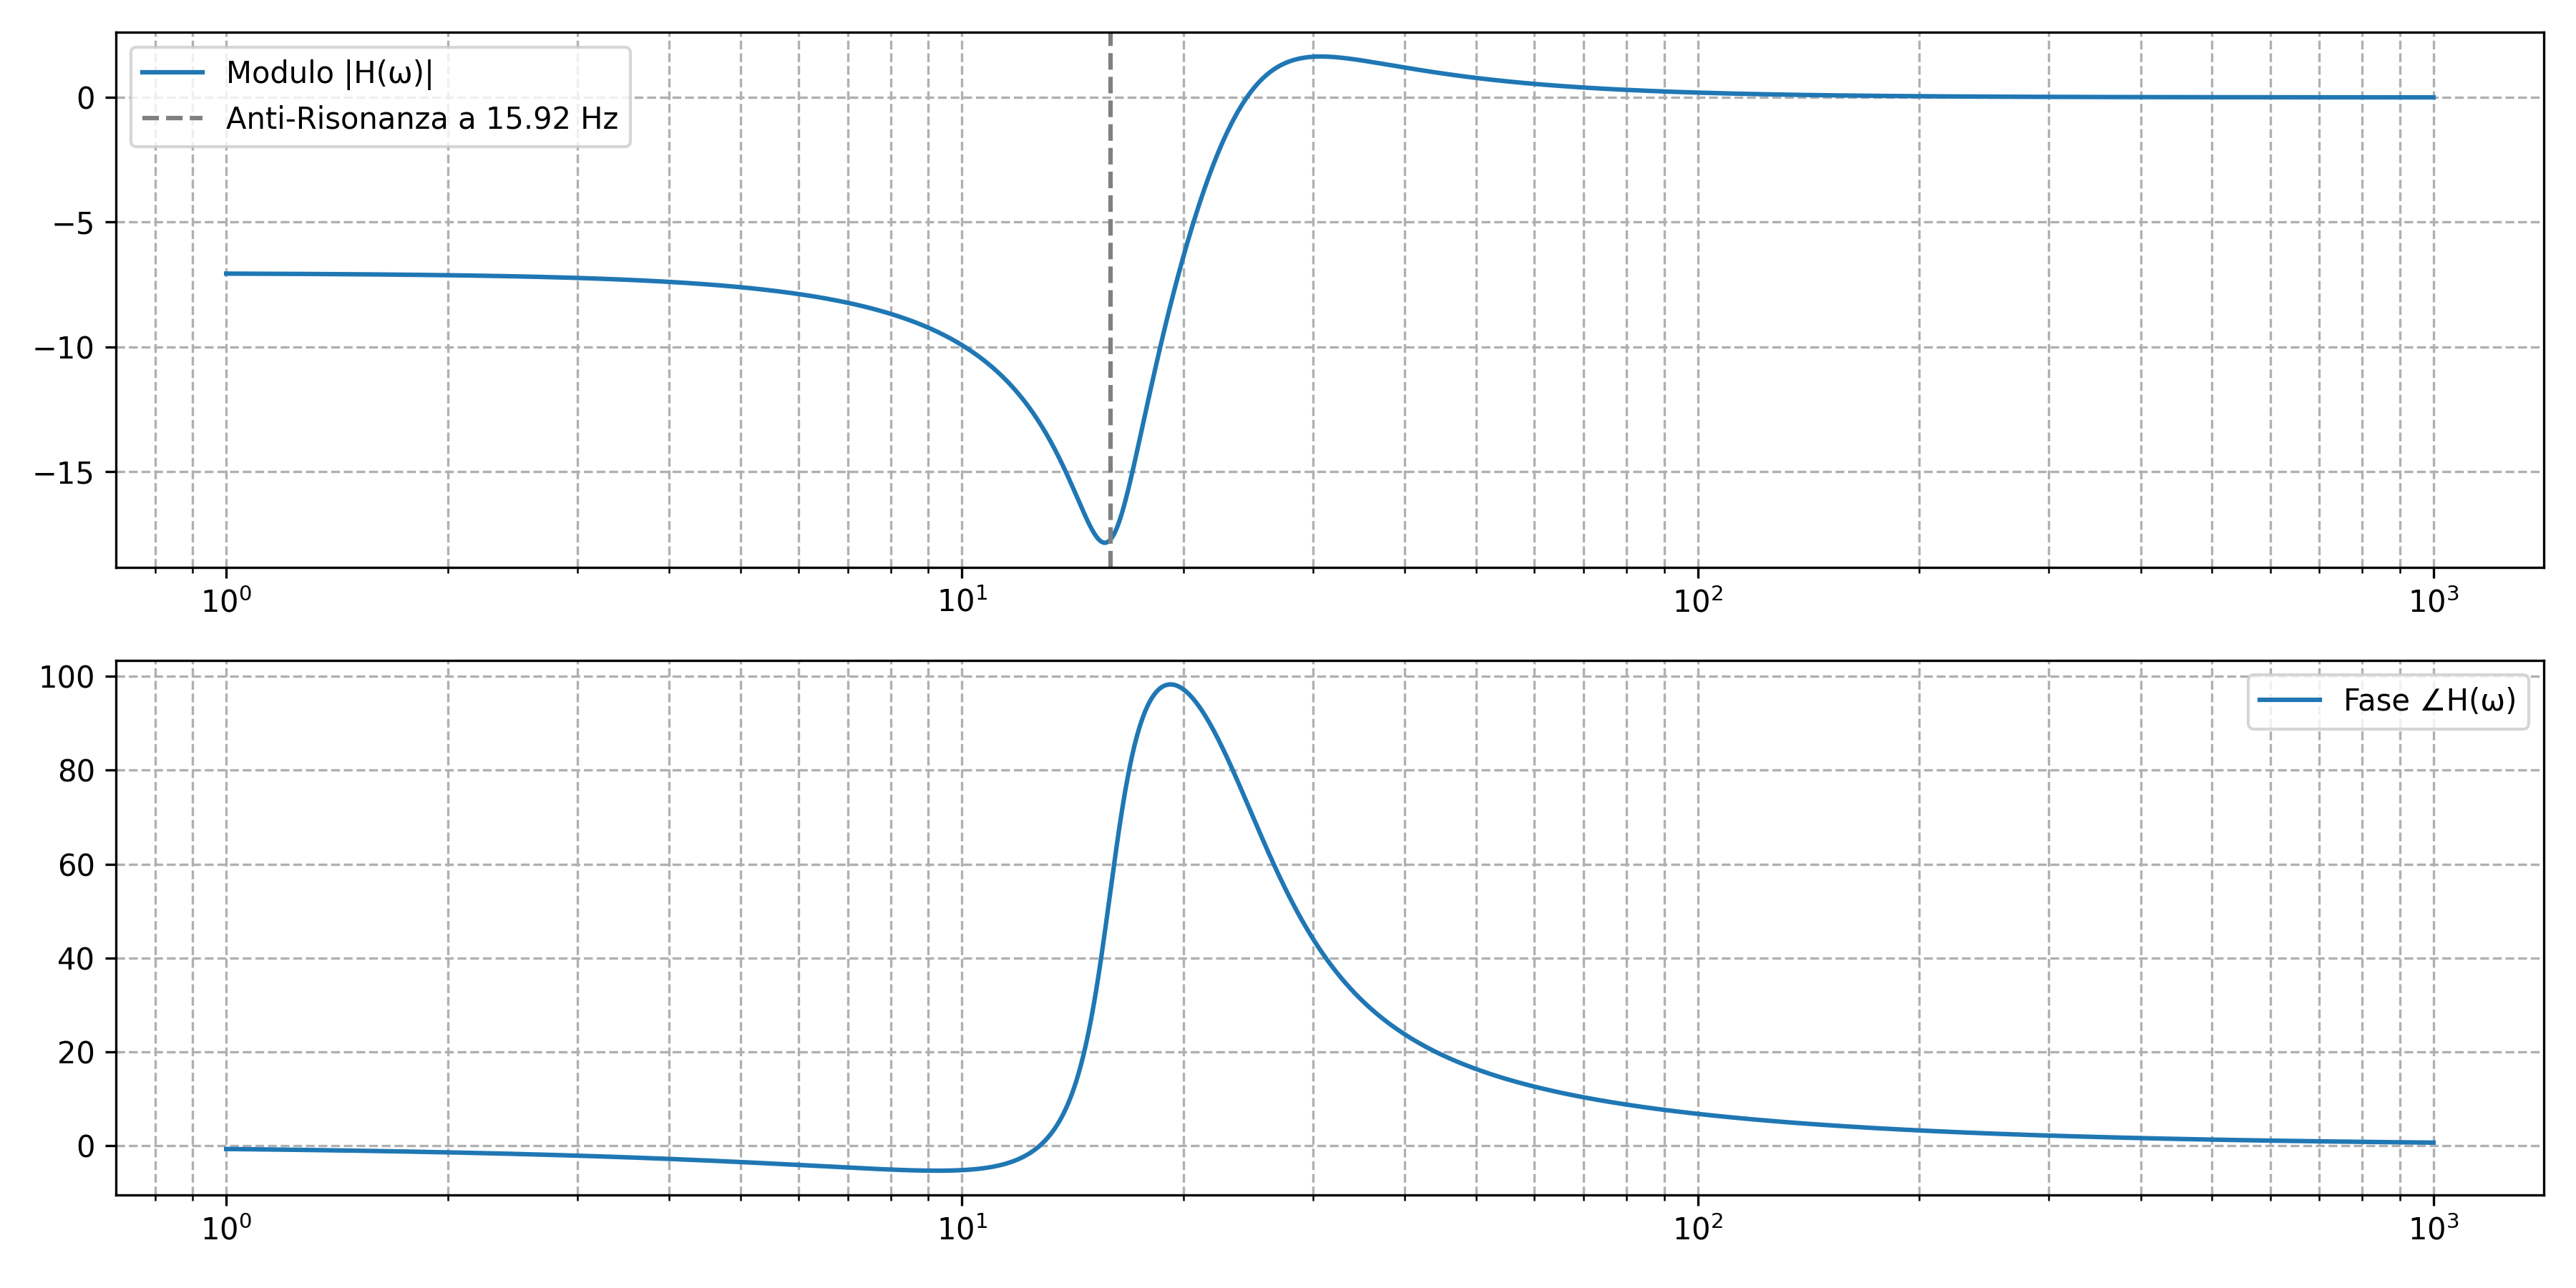
\includegraphics[width=0.5\textwidth]{Immagini/esempio_antirisonanza.png}
    \caption{Esempio di antirisonanza}
\end{figure}



% inserire figura di esempio, telaio, molla 1, massa 1, molla 2, massa 2 e massa 2 libera